\documentclass[
  a4paper,            % DIN A4
  DIV=10,             % Schriftgröße und Satzspiegel
  oneside,            % einseitiger Druck
  BCOR=5mm,           % Bindungskorrektur
  parskip=half,       % Halber Abstand zwischen Absätzen
  numbers=noenddot,   % Kein Punkt hinter Kapitelnummern
  bibtotoc,           % Literaturverzeichnis im Inhaltsverzeichnis
  listof=totoc,       % Abbildungs- und Tabellenverzeichnis im Inhaltsverzeichnis
  table
]{scrreprt}
\usepackage{../style/thesisstyle}

\makeglossaries           % create all glossary entries (remember: run makeglossaries manually)
\loadglsentries{thesisglossaries.tex}  % load acronym, symbol and glossary entries

\sisetup{locale = DE}     % siunitx locale setup
%\DeclareSIUnit \fps{fps}  % a custom unit (usage: \SI{24}{\fps})

\begin{document}
% !TEX root = ../thesis.tex
%
% configurations
%

% English Language support
% -> uncomment if needed
% Beta!
%\fullenglish{yes}
\fullenglish{no}

% text field
%-> replace supervisor names with correct ones
\firstSupervisor{Prof. Dr. Philipp Jenke}
\secondSupervisor{Prof. Dr. Peer Stelldinger}

% text field
%-> replace title with your thesis title
\thesisTitle{Beispiel-basierte inverse prozedurale Generierung für zweidimensionale Szenen}
\thesisTitleEN{Example-based inverse procedural generation for two-dimensional scenes}

% text field
%-> replace the key words with your own key words
\keywordsDE{TODO SCHLÜSSELWÖRTER}
\keywordsEN{TODO KEYWORDS}

% text field
%-> replace the text with a description of the thesis
\abstractDE{TODO ZUSAMMENFASSUNG}
\abstractEN{TODO ABSTRACT}

% text field
%-> replace john with your name
\thesisAuthor{Benjamin Schröder}

% text field
%-> enter the submission date
\submissionDate{11. Juli 2024}

% switch - uncomment only one
%-> uncomment NDA or public
%\NDA{yes}
\NDA{no}

% switch - uncomment only one
%-> uncomment old standard cover or cover Corporate Design 2017
\Cover{CD2017}
%\Cover{CD2017NoLogo}
%\Cover{Std2018}
%\Cover{Std2018_green} 			% with green bar

% switch - uncomment only one
%-> uncomment to show list of figures or not
\ListOfFigures{yes}
%\ListOfFigures{no}

% switch - uncomment only one
%-> uncomment to show list of tables or not
\ListOfTables{yes}
%\ListOfTables{no}

% switch - uncomment only one
%-> uncomment to show list of accronyms or not
\ListOfAccronyms{yes}
%\ListOfAccronyms{no}

% switch - uncomment only one
%-> uncomment to show list of symbols or not
\ListOfSymbols{yes}
%\ListOfSymbols{no}

% switch - uncomment only one
%-> uncomment to show list of glossary entries or not
\Glossary{yes}
%\Glossary{no}

% switch - uncomment only one
%-> uncomment the study course you are in
%\studycourse{ITS}
%\studycourse{TI}
\studycourse{AI}
%\studycourse{WI}
%\studycourse{EI}
%\studycourse{REE}
%\studycourse{BMP}		
%\studycourse{BMP-hp}	 % Internship Report in M&P
%\studycourse{BMT}
%\studycourse{BMT-st}    % Study / home assignment in BMT
%\studycourse{BMT-hp}    % Internship Report in BMT
%\studycourse{MI}
%\studycourse{MIK}
%\studycourse{MA}

\def\imgHeight{100pt}
\def\imgWidth{420pt}
    % load all settings

\hyphenation{Ba-che-lor-the-sis Mas-ter-the-sis}

% Cover page here, no page number
\ICoverPage

% PDF Metadata
% !TEX root = ../thesis.tex
%
% PDF Metadata integration
% @author Thomas Lehmann
%

% PDF Metadata
\hypersetup{
pdftitle={\IthesisTitle},
pdfauthor={\IthesisAuthor},
pdfkeywords={\IkeyWordsEN}
}

% Titlepage is page one even if the number is not shown.
\pagenumbering{roman}
% Title page here
% !TEX root = ../thesis.tex
%
% title page
% @author Thomas Lehmann
% Hints for title page and page numbering: https://en.wikipedia.org/wiki/Title_page
%
\title{\IthesisTitle}   % set latex default title to be used by hyperref in pdf
\author{\IthesisAuthor} % set latex default author to be used by hyperref in pdf

\newpage
\thispagestyle{empty}
{\fontfamily{phv}\selectfont
  \hfuzz=20pt       % suppress warnings due to extension onto page margins

  % Author of thesis
  \vspace*{1cm}
  \begin{minipage}[b]{\textwidth}
    \fontsize{14pt}{20pt}
    \selectfont
    \begin{center}
      \IthesisAuthor
    \end{center}
  \end{minipage}

  % Title of thesis
  \vspace{1.5cm}
  \begin{minipage}[b][0cm][t]{\textwidth}
    \fontsize{18pt}{20pt}
    \selectfont
    \begin{center}
      \IthesisTitle
    \end{center}
  \end{minipage}

  % Important information
  \begin{textblock*}{\textwidth}(40mm,210mm)
    \begin{minipage}[b]{\textwidth}
      \hbadness=10001    % suppress underfull warning due to short text
      \fontfamily{cmr}\selectfont
      \fontsize{12pt}{14pt}
      \selectfont
      \ifdefined\ILanguageEN
        \IthesisKindEN ~submitted for examination in \IthesisExaminationEN \\
        in the study course \textit{\IstudyCourseName} \\
        at the \IthesisDepartmentFullEN \\
        at the \IthesisFacultyFullEN \\
        at University of Applied Science Hamburg\\

        Supervisor: \IfirstSv \\
        \ifdefined\IisTermPaper
          % left blank
        \else
          \ifdefined\IisInternshipReport
	  Supervised: \IsecondSv\\
          \else
        Supervisor: \IsecondSv \\
          \fi\fi
        
        Submitted on: \ISubDate \\
      \else
      	\ifdefined\IisInternshipReport
        \IthesisKindDE ~eingereicht im Rahmen des \IthesisExaminationDE \\	
	\else
        \IthesisKindDE ~eingereicht im Rahmen der \IthesisExaminationDE \\
        \fi
	im Studiengang \textit{\IstudyCourseName} \\
        am \IthesisDepartmentFull \\
        der \IthesisFacultyFull \\
        der Hochschule für Angewandte Wissenschaften Hamburg\\

        Betreuender Prüfer: \IfirstSv \\
        \ifdefined\IisTermPaper
          % left blank
        \else
          \ifdefined\IisInternshipReport
        betriebliche Betreuung: \IsecondSv \\							
	  \else
        Zweitgutachter: \IsecondSv \\
        \fi\fi

        Eingereicht am: \ISubDate \\
      \fi
    \end{minipage}
  \end{textblock*}
}


% Abstract page here
% !TEX root = ../thesis.tex
%
% abstract page
% @author Thomas Lehmann
%
\newpage
\thispagestyle{plain}
\clearpage
\hfuzz=12pt       % suppress warnings due to extenstion onto page margins

\textbf{\IthesisAuthor}

\vspace{0.3cm}
\textbf{Thema der Arbeit}

\IthesisTitle

\vspace{0.3cm}
\textbf{Stichworte}

\IkeyWordsDE

\vspace{0.3cm}
\textbf{Kurzzusammenfassung}

\begin{minipage}{\textwidth}
\IabstractDE
\end{minipage}

\vspace{1.0cm}
\textbf{\IthesisAuthor}

\vspace{0.3cm}
\textbf{Title of Thesis}

\IthesisTitleEN

\vspace{0.3cm}
\textbf{Keywords}

\begin{minipage}{\textwidth}
\IkeyWordsEN
\end{minipage}

\vspace{0.3cm}
\textbf{Abstract}

\IabstractEN


% Table of contents here
\tableofcontents

% List of figures here
\IListOfFigures

% List of tables here
\IListOfTables

% List of accronyms here
\IListOfAccronyms

% List of symbols here
\IListOfSymbols

% Uncomment if list of source code is needed (rarely).
%\lstlistoflistings  % requires package listings, needs to uncommenting of usepackage

% path to the chapters folder is set to find the images used there
\graphicspath{ {./chapters/} }

% Chapters
\clearpage
\pagenumbering{arabic}
% @author Benjamin Schröder
%
\chapter{Einleitung}

\section{Motivation}
% In diesem Abschnitt wird erklärt, wieso die prozedurale Generierung überhaupt so ein wichtiges Thema ist.
% Es wird geklärt, wer davon Gebrauch macht, und wieso es für den entsprechenden Anwender Sinn macht. Dazu zählt
% zum Einen das Einsparen von Ressourcen, aber auch das Umsetzen von Spielkonzepten, die durch die hier vorgestellten
% Verfahren erst möglich werden.
Die Erstellung von fiktiven Welten spielt eine große Rolle in vielen Videospielen, Filmen, Virtual Reality Umgebungen
und weiteren Bereichen der Simulation. Hierfür wird eine Vielzahl an verschiedenen Objekten und Strukturen benötigt, um
ein nicht-repetitives und immersives Erlebnis für den Endnutzer zu schaffen. All dies manuell anzufertigen, stellt vor
allem kleinere Indie-Entwicklerstudios vor eine große Herausforderung und kann die Entwicklungszeit signifikant in die
Länge ziehen. Aber auch in größeren Teams mit einer Vielzahl von Designern nimmt die Erstellung von realistischen Welten einen
Großteil der Entwicklungszeit in Anspruch und kann viele Monate dauern. \cite{10_freiknecht} Hier kann an einigen Stellen
nachgeholfen werden, indem man das Erstellen von Inhalten automatisiert. Entsprechende Prozesse lassen sich dem Bereich
der prozeduralen Generierung zuordnen.

Mithilfe von verschiedensten Verfahren können so z.B. einzelne Dungeons oder sogar ganze Welten und darin enthaltene Gebilde
automatisch erzeugt werden. Diese können eine Grundstruktur für ein komplexeres Design bilden, bei dem die Entwickler dann nur noch
kleinere Details per Hand abändern oder hinzufügen müssen. \cite{10_freiknecht} Andererseits existieren auch viele Videospiele,
wie z.B. Minecraft\footnote{\url{https://www.minecraft.net/} [Letzter Zugriff am 01.07.2024]} oder Terraria\footnote{
\url{https://terraria.org/} [Letzter Zugriff am 01.07.2024]}, die auf prozeduraler
Generierung aufbauen, um ihr Spielkonzept umzusetzen. Konkret wird einem neuen Spieler hier eine komplett neue und einzigartige,
aber dennoch logisch zusammenhängende Welt generiert; dies vollautomatisch und ohne zusätzlichen Aufwand für die Entwickler. Jeder
Spieler bekommt so eine einzigartie Erfahrung geboten und kann das Spiel außerdem gewissermaßen unbegrenzt oft durchspielen, ohne
dass es zu repetitiv wird. So etwas wäre ohne Automatisierung gar nicht erst umsetzbar.

\section{Problemstellung}
% Hier wird dann darauf aufmerksam gemacht, dass es bei diesen Verfahren viele Limitationen gibt. Bei vielen Verfahren
% ist es nötig, manuell Regeln für den Algorithmus zu erstellen, sodass dieser überhaupt arbeiten kann. Dies setzt wiederum
% einiges an Kenntnissen voraus und ist somit nicht für jeden zugänglich. Außerdem werden weitere Probleme aufgezeigt.

% Alte Formulierung:
% Es gibt viele bekannte Verfahren, welche solche Ergebnisse unter der Verwendung von u.a. zellulären Automaten, generativen
% Grammatiken oder Constraint-basierten Graphen erzielen können. \cite{5_van_der_linden_et_al} Ein Großteil dieser Verfahren erfordert jedoch
% menschliches Eingreifen in einigen der Teilschritte. So z.B. muss beim Verwenden einer generativen Grammatik meist bereits eine Menge
% an Produktionsregeln durch einen Menschen vorgegeben werden, bevor die automatische Generierung überhaupt beginnen kann. Das Erstellen
% solcher Regeln ist mit viel Arbeit und Trial-and-Error verbunden und kann ohne ein ausgeprägtes Verständnis des angewandten Verfahrens
% sehr schwierig werden. Dadurch kommt es für viele Designer letztendlich doch nicht in Frage. Auch gibt es Szenarien, in denen die Generierung
% von Inhalten durch den Endnutzer beeinflusst werden kann, so z.B. in Spielen, in denen der Spieler dynamisch mit dem Terrain und anderen
% Strukturen interagieren kann. In einem solchen Fall kann der Entwickler keinen direkten Einfluss auf den Generierungsprozess nehmen und alles
% muss voll automatisiert sein. \cite{14_carli_et_al} Hier setzt diese Arbeit an und untersucht Möglichkeiten zur vollständigen Automatisierung
% solcher Verfahren.

Es gibt viele bekannte Verfahren, welche solche Ergebnisse unter der Verwendung von u.a. generativen
Grammatiken oder Constraint-basierten Graphen erzielen können. \cite{5_van_der_linden_et_al} Ein Großteil dieser Verfahren erfordert jedoch
menschliches Eingreifen in einige der Teilschritte, was in einigen Szenarien zu einem Problem werden kann. Hängt die Generierung von
Inhalten eines Produkts z.B. von Entscheidungen des Endnutzers ab (z.B. in Spielen, in denen der Spieler dynamisch mit
dem Terrain und anderen Strukturen interagiert), so kann der Entwickler keinen direkten Einfluss auf den Generierungsprozess
nehmen und alles muss voll automatisiert sein. \cite{14_carli_et_al} Auch in Projekten, in denen dies nicht der Fall ist und der gesamte Inhalt
im Voraus erstellt wird, kann das Voraussetzen von menschlicher Intervenierung als Teil des Prozesses zu einem Problem werden.
Ein Beispiel hierfür wären Verfahren, die eine generative Grammatik nutzen und voraussetzen, dass dafür zunächst eine Menge an Regeln
durch einen Menschen vorgegeben wird, bevor die automatische Generierung überhaupt beginnen kann (z.B. \cite{33_adams}\footnote{
\url{https://citeseerx.ist.psu.edu/document?repid=rep1&type=pdf&doi=25020f8d955aee07b7dd49a3ec23b1f2a8cf1d06} [Letzter Zugriff am 01.07.2024]}).
Das Erstellen solcher Regeln ist mit viel Arbeit verbunden und kann ohne ein ausgeprägtes Verständnis des angewandten Verfahrens sehr
schwierig werden, wodurch der Einsatz eines solchen Verfahrens für viele Designer letztendlich doch nicht in Frage kommen wird. Hier
setzt diese Arbeit an und untersucht Möglichkeiten zur Automatisierung des Erstellens solcher Regeln.

\section{Ziele und Vorgehen}
% Aus den aufgezeigten Problemen ergibt sich nun der Sinn dieser Arbeit. Inverse Verfahren beheben die oben genannten Probleme
% und sollen deswegen genauer untersucht werden. Es werden verschiedene Verfahren analysiert und miteinander verglichen.
% Anschließend wird ein entsprechendes und vielversprechendes Verfahren im Detail untersucht, theoretisch erläutert und
% dann prototypisch implementiert.
Spezifisch soll versucht werden, Muster in Beispielstrukturen zu identifizieren. Aus diesen Mustern sollen dann Regeln zum Zusammensetzen
von Strukturen mit ähnlichen Eigenschaften abgeleitet werden. Gelingt dies, so muss ein Designer lediglich ein einziges Beispielmodell erstellen und
kann damit eine kreative Vision vorgeben. Alle weiteren Schritte zum Ableiten von Variationen dieses Inputs laufen anschließend automatisch ab.
Dies nennen wir \textit{inverse} prozedurale Generierung,
da der Prozess mit einem soweit fertigen Modell beginnt und daraus dann die Regeln ableitet, statt wie in den klassischen Verfahren zuerst mit
der Erstellung der Regeln zu beginnen. Die Erstellung eines Beispielmodells erfordert zwar nach wie vor die Arbeit eines Designers, anschließend
ist aber kein menschliches Eingreifen mehr nötig und das eigentliche Verfahren läuft vollautomatisch ab.

Es gibt bereits verschiedene Verfahren, die einen solchen Ansatz verfolgen. Diese sind u.a. der Gitter-basierte Wave Function
Collapse Algorithmus von Maxim Gumin \cite{45_gumin} oder die nach Symmetrien suchende inverse prozedurale Modellierung von Bokeloh
et al. \cite{3_bokeloh_et_al}.

Im Rahmen dieser Arbeit werden entsprechende Verfahren grob analysiert, deren Probleme aufgezeigt und anschließend ein neuer Ansatz vorgestellt,
welcher die vorhandenen Probleme minimieren soll. Das Endergebnis der Arbeit soll dann sein, dass die Funktionsweise des neuen Konzepts
ausführlich und verständlich dargestellt, und dieses anschließend prototypisch implementiert wird. Wir begrenzen uns dabei auf die Generierung von
Strukturen im zweidimensionalen Raum. Der gleiche Ansatz kann auch auf den dreidimensionalen Raum erweitert werden, um so vielseitiger einsetzbar zu
sein, jedoch reicht die vereinfachte Betrachtung zum Darstellen aller fundamentalen Konzepte.
% @author Benjamin Schröder
%
\chapter{Grundlagen}
In diesem Kapitel werden einige grundlegende Konzepte behandelt, welche zum Verständnis dieser Arbeit beitragen. Zunächst wird
erklärt, was genau unter dem Begriff der prozeduralen Generierung zu verstehen ist, woraufhin einige der fundamentalen Verfahren
vorgestellt werden.

\section{Prozedurale Generierung}
Prozedurale Generierung, oft auch \gls{ac:pcg}, beschreibt eine Menge von Verfahren zum
algorithmischen Erstellen von Inhalten ("Content"). Dabei handelt es sich meist um Verfahren, die automatisch Texturen
oder verschiedene Gebilde im Kontext von Videospielen erzeugen können, so z.B. Landschaften, Flüsse, Straßennetze,
Städte oder Höhlenstrukturen. Auch Musik kann durch solche Verfahren generiert werden, was für diese Arbeit allerdings
weniger relevant ist. \cite{9_togelius_et_al}

TODO:
- Eingehen auf Zufälligkeit \& deterministisches Verhalten (Reproduzierbarkeit durch Seed) -> Quelle 9
- Eingehen auf Unterscheidung zwischen assisted/non-assisted -> Quelle 14

- Auf Begriffe Prozedural, Content, und Generierung einzeln eingehen ?

Diese Definition ist absichtlich etwas allgemeiner gehalten, da das Aufstellen einer spezifischeren Definition nicht
besonders trivial ist. Das Konzept von \gls{ac:pcg} wurde bereits aus vielen veschiedenen Blickwinkeln beleuchtet und ist für verschiedene
Personen von unterschiedlicher Bedeutung. So hat z.B. ein Game Designer eine etwas andere Perspektive als ein Wissenschaftler, der
sich lediglich in der Theorie mit der Thematik beschäftigt. Verschiedene Definitionen unterscheiden sich in Bezug auf
Zufälligkeit, die Bedeutung von "Content", oder darin, ob und in welchem Umfang menschliche Intervenierung eine Rolle in einem
Verfahren spielen darf. Mit diesem Problem haben sich Togelius et al. \cite{9_togelius_et_al} bereits ausführlich befasst, weshalb dies hier
nicht weiter thematisiert werden soll. Für diese Arbeit soll die oben genannte Definition ausreichen.

\section{Verwendung von PCG}
% evtl. weglassen?
Da die Entwicklung von Videospielen aufgrund der großen Anzahl an benötigten Inhalten sehr schnell sehr aufwändig werden
kann, findet \gls{ac:pcg} vor allem in dieser Industrie einen großen Nutzen. Gerade das Erstellen von immersiven Welten erfordert eine Vielzahl
von verschiedensten detaillierten Modellen und kann manuell nur mit sehr großem Arbeitsaufwand umgesetzt werden. Das Automatisieren der
Generierung von Inhalten kann den Entwicklerstudios hier eine bedeutende Menge an Zeit und Kosten sparen, die dann an anderen
Stellen eingesetzt werden können. In vielen Fällen kann sogar Speicherplatz gespart werden, indem die Generierung der Inhalte
zur Laufzeit stattfindet.

\gls{ac:pcg} hat bereits in vielen bekannten Videospielen Verwendung gefunden. Schon im Jahr 1980 wurde %rogue

TODO: Aufzählen von Spielen mit PCG Algorithmen

\section{Perlin Noise}
Ein fundamentales Konzept im Bereich von \gls{ac:pcg} ist das Verwenden von Rauschfunktionen, oder auch \textit{Noise}.
Der wohl bekannteste Vertreter dieses Konzepts ist das 1985 von Ken Perlin entwickelte \cite{16_perlin} und 2002 verbesserte \cite{18_perlin}
\textit{Perlin Noise}, welches seit dessen Veröffentlichung nicht mehr aus der Welt der Computergrafik wegzudenken ist. Mithilfe von
Perlin Noise können eine Reihe von Zufallswerten erzeugt werden. Hierbei sind sich nah beieinander liegende Werte stets sehr ähnlich und es
gibt keine starken Ausschläge, weshalb der entstehende Verlauf sehr organisch wirkt. Aufgrund von dieser Eigenschaft eignet sich Perlin Noise
perfekt zum Erzeugen von natürlichen Strukturen wie z.B. Hügellandschaften oder Inselgruppen. Generell ist der erzeugte Kurvenverlauf vielseitig
einsetzbar und findet somit in vielen verschiedenen Anwendungen einen Nutzen, darunter auch im Bereich der Animation. \cite{17_lagae_et_al}

TODO: Einfügen von Vergleich zwischen Random Noise und Perlin Noise

Neben der vielseitigen Einsetzbarkeit von Perlin Noise gibt es außerdem den Vorteil, dass dieses Verfahren sehr günstig sowohl in Bezug auf
die Berechnungszeit als auch in Bezug auf die Speicherverwendung ist. Einzelne Punkte im Verlauf lassen sich unabhängig voneinander berechnen,
wodurch sich der Berechnungsprozess wunderbar parallelisieren lässt. Dies wird mit der immer weiter voranschreitenden Entwicklung von
Grafikkarten und Prozessoren auch zu einem immer größeren Vorteil. \cite{17_lagae_et_al}

Perlin Noise kann für eine beliebige Anzahl an Dimensionen berechnet werden. Dazu wird der n-dimensionale Raum in eine reguläre gitterartige
Struktur aufgespalten. Die Punkte auf dem Gitter sind dabei all jene, die an ausschließlich ganzzahligen Koordinaten liegen. Im zweidimensionalen
Raum wäre dies also die Menge an Punkten \(\{(x, y) \ \| \ x, y \in \mathbb{N}\}\). Alle anderen Punkte im Raum befinden sich dann jeweils innerhalb
einer der von den Gitterpunkten aufgespannten Zellen.

\begin{figure}[h]
    \centering
    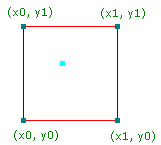
\includegraphics[height=\imgHeight]{images/noise_cell.png}
    \caption{Beispiel einer Gitterzelle im 2D}
    \label{fig:noise_cell}
\end{figure}

Jeder der Gitterpunkte bekommt außerdem einen pseudozufälligen Gradienten (Richtungsvektor der Länge 1) zugeordnet.

\begin{figure}[h]
    \centering
    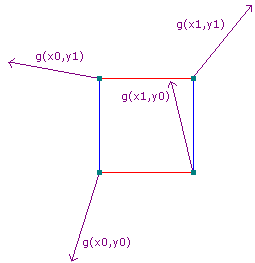
\includegraphics[height=\imgHeight]{images/noise_gradient.png}
    \caption{Pseudozufällige Gradienten für die Eckpunkte einer Zelle im 2D}
    \label{fig:noise_gradient}
\end{figure}

Soll jetzt der Noise-Wert
für einen Punkt im Raum berechnet werden, werden zunächst die Eckpunkte der betroffenen Zelle und deren zugeordnete Gradienten ermittelt.
Außerdem werden die Vektoren berechnet, die von den Eckpunkten in Richtung des aktuellen Punktes zeigen.

\begin{figure}[h]
    \centering
    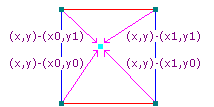
\includegraphics[height=\imgHeight]{images/noise_vectors.png}
    \caption{Vektoren von den Eckpunkten zu einem Punkt im Inneren einer Zelle im 2D}
    \label{fig:noise_vectors}
\end{figure}

Anschließend wird dann für jeden Eckpunkt
das Skalarprodukt aus dem dortigen Gradienten und dem Vektor in Richtung des Punktes gebildet. Der Mittelwert all dieser Skalarprodukte ergibt
dann den finalen Noise-Wert. \cite{16_perlin}\footnote{Erklärung in Anlehnung an https://mzucker.github.io/html/perlin-noise-math-faq.html}

TODO: Erklärung mathematisch beschreiben, Abbildungen erneuern/in eine Abbildung zusammenfassen

\section{L-Systeme}
Ein weiteres bekanntes Konzept ist das der L-Systeme.

\section{Fraktale}
\cite{19_mandelbrot_frame}




example-based model synthesis -> (weitere Merrell Verfahren) -> wave function collapse -> example-based procedural modeling using graph grammars
% @author Benjamin Schröder
%
\chapter{Theorie}
Im Folgenden werden die theoretischen Konzepte hinter dem praktischen Teil der Arbeit betrachtet. Das implementierte Verfahren wird
Schritt für Schritt vorgestellt und im Detail erläutert. Die vorgestellten Konzepte beruhen auf den Erkenntnissen von Paul Merrell
in seiner Arbeit aus dem Jahr 2023 \cite{1_merrell}.

% Konzepte:
% - Graphen, Graph-Grammatiken, Graphersetzungssysteme (Erstellen von Regeln), Graphisomorphismen (Anwenden von Regeln)
% - Local Similarity
% - Einfärben von Facetten
% - Facetten-Label
% - Kanten-Label (gleiche anliegenden Farben, gleicher Tangentenwinkel)
% - Kanten, Halbkanten
% - Teilen (Cut-Operation) und Zusammenkleben (Branch \& Loop Gluing) von Kanten
% - Vollständige \& unvollständige Graphen
% - Planarität
% - Positive \& negative turns
% - Graph Boundary String
% - Einfachheit/Simplicity von Graphen
% - Reduzierbarkeit (reducible graphs)
% - Irreducible Graphs (alle Graphen sind entweder reduzierbar oder unvollständig)
% - (Lösen von LGS zum Bestimmen der Knotenpositionen)

\section{Überblick}
% - Beispielstruktur als Input (Graph)
% - Aufteilen in Primitives (Teilen von Kanten in Halbkanten)
% - Primitives in allen möglichen Wegen zusammenkleben zum Erstellen von Hierarchie
% - Erstellen von Graph-Grammatik aus Hierarchie (im Idealfall können hiermit dann alle locally similar Graphen erstellt werden)
% - Ableiten von neuen Graphen aus der Grammatik
% - Festsetzen von Knotenpositionen des Graphen, um die letztendliche Geometrie zu erhalten
% - Optional: Dekorieren/Texturieren der erhaltenen Geometrie (wahrscheinlich nicht direkt relevant für diese Arbeit)

Bevor es um die Einzelheiten und spezifischen Konzepte geht, wird zunächst ein grober Überblick zum Ablauf des umgesetzten
Verfahrens geliefert. Das Ganze beginnt mit einer polygonalen Inputstruktur, d.h. einem Gebilde bestehend aus einem oder mehreren Polygonen.
Diese Inputstruktur wird anschließend umgewandelt in einen Graphen, in welchem die Punkte des Polygons als Knoten und die Verbindung zwischen
den Punkten als Kanten dargestellt werden. Die Darstellung als Graph ist nützlich, da in dieser die konkrete Geometrie des Inputs keine Rolle
mehr spielt und sich auf die für das Verfahren wichtigen Eigenschaften des Inputs konzentriert werden kann.

Im nächsten Schritt wird der erstellte Graph nun in seine kleinstmöglichen Einzelteile zerlegt. Dazu werden alle Kanten in zwei Halbkanten
aufgeteilt. Das Ergebnis sind viele Teilgraphen, welche jeweils nur noch aus einem Knoten und einigen Halbkanten bestehen. Einen solchen Teilgraphen
nennen wir \textit{Primitiv}. Diese Primitive werden dann Schritt für Schritt in allen möglichen Kombinationen zusammengeklebt, was zum Entstehen
einer Hierarchie an immer komplizierter werdenden Graphen führt. Beim Aufbau der Hierarchie werden die neu entstehenden Graphen auf bestimmte
Eigenschaften überprüft, die es uns erlauben, daraus Regeln für ein Graphersetzungssystem abzuleiten. Das einfachste Beispiel hierfür sind
vollständige Graphen, also Graphen, die nur noch aus in sich geschlossenen Kreisen bestehen und keine Halbkanten mehr besitzen. Aus diesen lässt
sich eine sogennante Startregel ableiten, welche den leeren Graphen mit dem gefundenen vollständigen Graphen ersetzt. Das Finden von weiteren
Regeln ist deutlich komplizierter und wird später im Detail erläutert.

% TODO: Bild von Startregel

Sobald man nun eine Menge von Regeln für das Graphersetzungssystem gefunden hat, kann man diese verwenden um verschiedenste zum Inputgraphen
ähnliche Graphen abzuleiten, indem zufällig verschiedene Regeln nach und nach angewendet werden. Für einen solchen Graphen müssen dann noch
konkrete Knotenpositionen und Kantenlängen bestimmt werden, sodass dieser wieder als Struktur aus Polygonen dargestellt werden kann. Hier
findet das Verfahren schließlich auch sein Ende.

\section{Input}
Der Algorithmus kann mit beliebigen polygonalen Strukturen als Input arbeiten. Dies können einfache Rechtecke oder aber auch komplizierte Gebilde
aus verschiedenen Häusern oder ähnlichem sein. Wichtig ist lediglich, dass der Input als Sammlung von Punkten und Kanten beschrieben werden kann.
So sind z.B. Kreise oder andere Strukturen mit Rundungen kein valider Input und können wenn dann nur durch komplexe Polygone angenähert werden.

Zur Verarbeitung des Inputs wird dieser in einen Graphen umgewandelt, in welchem die spezifischen Positionen der Knoten keine Rolle spielen.
Stattdessen wird nur abgebildet, welche Knoten es überhaupt gibt, welche der Knoten durch Kanten miteinander verbunden sind, und in welchem Winkel
diese Kanten verlaufen. Außerdem können die einzelnen Polygone mit Farben versehen werden, um verschiedene abgegrenzte Bereiche zu markieren.
Die Kanten im Graphen werden mit einem entsprechenden Label versehen, welches neben den Start- und Endknoten ebenfalls Informationen zum
Tangentenwinkel, sowie zu den Farben der links und rechts anliegenden Polygone enthält. Ein Kantenlabel besitzt die Form
\(\tilde{a} = (l,r,\theta)\), wobei \(\tilde{a}\) die Bezeichnung der Kante, \(l\) und \(r\) die Farben der anliegenden Polygone, und
\(\theta\) der Tangentenwinkel der Kante sind.

\section{Lokale Ähnlichkeit}
Ziel des Algorithmus ist es, Variationen des Inputs zu erzeugen. Dabei soll der Output eine gewisse Ähnlichkeit zum Input beibehalten. Global
vorzugehen und die vollständigen Input- und Output-Strukturen miteinander zu vergleichen führt hierbei allerdings zu keinem vernünftigen
Ergebnis. Der Output muss sich zwingend vom Input unterscheiden, ansonsten ist das Ergebnis nicht zu gebrauchen. Um Vergleiche auf einer kleineren
Ebene vornehmen zu können, stellen wir hier das Konzept der \textit{lokalen Ähnlichkeit} vor.
% @author Benjamin Schröder
%
\chapter{Implementation}
% @author Benjamin Schröder
%
\chapter{Auswertung}
\label{chap:auswertung}
Werten wir die vorgestellte Implementierung nun aus. Dazu überprüfen wir zunächst die anfangs vorgestellten Anforderungen an die gesamte
Software und diskutieren anschließend, wie erfolgreich dabei das eigentliche Verfahren umgesetzt wurde. Dazu werden einige
Beispieldurchläufe mit verschiedenen Parameter-Werten betrachtet.

\section{Überprüfen der Anforderungen}
\subsection{Funktionale Anforderungen}
\subsubsection{Funktionale Anforderung 1}
\textit{Es sollen beliebige polygonale 2D-Strukturen als Input eingelesen werden können.} Diese Anforderung wird
durch die entwickelte \code{PolygonMesh} Datenstruktur realisiert. In dieser können beliebige Polygone in eine größere zusammenhängende
Struktur gebracht werden. Diese Datenstruktur kann von der \code{GrammarBuilder} Klasse als Input entgegengenommen werden, was die
Grundlage für das Durchführen aller weiteren Teilschritte des Verfahrens darstellt.

\subsubsection{Funktionale Anforderung 2}
\textit{Es sollen einige Beispielstrukturen als Input zur Verfügung gestellt werden, zwischen denen der Nutzer auswählen kann.}
Dies wird durch die vorgestellte \code{InputScene} realisiert. Hier kann der Benutzer ein Dropdown-Menü öffnen und erhält eine Liste an
möglichen Beispielstrukturen, die alle vom \code{InversePcgController} in ein \code{PolygonMesh} Objekt umgewandelt werden können.
Beispielstrukturen können ohne viel Aufwand und ohne Anpassung des Codes entfernt, hinzugefügt oder ausgetauscht werden, da diese in
separaten \code{.mesh}-Dateien gespeichert werden und dynamisch zur Laufzeit eingelesen werden können.

\subsubsection{Funktionale Anforderung 3}
\textit{Es sollen automatisch zum Input lokal ähnliche Strukturen generiert werden können.} Die Theorie hinter dem implementierten Verfahren beruht
vollständig auf den in \autoref{chap:konzept} vorgestellten Konzepten und erzeugt den Output nach dem dort beschriebenen Vorgehen. Ist das Verfahren
erfolgreich durchgelaufen, so lässt sich jeder Teil der dadurch erzeugten Outputstruktur im Input wiederfinden und die erzeugte Strukture ist somit
lokal ähnlich zum Input. In vielen Fällen kann das Verfahren aufgrund von Defiziten in der \code{MeshSolver} Komponente jedoch nicht erfolgreich durchlaufen,
wodurch diese Anforderung nicht immer vollständig erfüllt werden kann.

\textit{a) Aus einer eingelesenen Inputstruktur sollen automatisch Regeln für eine Graphgrammatik abgeleitet werden können.} Diese Anforderung wird
durch die Klasse \code{GrammarBuilder} realisiert, welche ein gegebenes \code{PolygonMesh} Objekt in eine \code{GraphGrammar} umwandeln kann.

\textit{b) Aus einer gegebenen Graphgrammatik sollen verschiedene Graphen abgeleitet werden können.} Hierfür ist die \code{GraphBuilder} Klasse zuständig.
Der dort entwickelte Algorithmus nimmt ein \code{GraphGrammar} Objekt entgegen und erzeugt daraus ein neues \code{AngleGraph} Objekt.

\textit{c) Aus einem solchen Graphen soll dann eine planare Outputstruktur mit fester Geometrie (also festen Knotenpositionen) erzeugt werden können.}
Dies wird vom \code{MeshSolver} übernommen, welcher ein \code{AngleGraph} Objekt in ein \code{PolygonMesh} Objekt umwandeln kann. Hier gibt es allerdings
das Problem, dass in vielen Fällen keine valide Lösung für die Outputstruktur gefunden werden kann. Bei der Verarbeitung etwas größerer Winkelgraphen
entstehen beim Lösen des entstandenen Gleichungssystems so viele freie Variablen, dass es eine ziemlich große Wahrscheinlichkeit gibt, dass zumindest
eine dieser Variablen zum Erzeugen von ungültigen Werten für eine der anderen unbekannten Variablen führt. Dies versuchen wir zu umgehen, indem
dieser Vorgang bis zu \code{maxTries} Mal wiederholt wird, in der Hoffnung, dass die jeweils nächste zufällige Lösung gültig sein wird. Da jedes Mal
jedoch alle Variablen erneut generiert werden, ist die Fehlerwahrscheinlichkeit dabei so hoch, dass in den meisten Fällen auch nach etlichen Versuchen
keine valide Lösung generiert werden kann. In diesem Fall visualisieren wir trotzdem die zuletzt erzeugte Struktur, jedoch wird diese nicht vollständig
zum Input lokal ähnlich sein.

\subsubsection{Funktionale Anforderung 4}
\textit{Es soll eine grafische Benutzeroberfläche geben, in welcher der Nutzer Parameter für die Generierung einstellen, sowie zwischen
den verschiedenen Inputstrukturen auswählen können soll.} Dies wird durch die Klasse \code{InversePcgApplication} realisiert. In den drei darin
implementierten Szenen kann der Nutzer alle wichtigen Einstellungen vornehmen. In der \code{InputScene} kann der Seed für den Zufallsgenerator festgelegt
und eine Inputstruktur ausgewählt werden. In der \code{GrammarScene} kann die Anzahl an Generation in der Graph-Hierarchie festgelegt werden. In der
\code{OutputScene} können alle weiteren in \autoref{chap:datenmodell} vorgestellten Parameter eingestellt werden.

\subsubsection{Funktionale Anforderung 5}
\textit{Sowohl die Inputstrukturen, die daraus erzeugt Grammatik und die generierten Variationen sollen visualisiert werden können.} Die Visualisierung
der hier genannten Datenstrukturen wird ebenfalls durch die \code{InversePcgApplication} übernommen. In der \code{InputScene} wird die ausgewählte
Inputstruktur dargestellt, die \code{GrammarScene} übernimmt das Darstellen der daraus erzeugten Grammatik, und die \code{OutputScene} wird zum
Visualisieren der verschiedenen erzeugten Variationen benutzt.

\subsection{Nichtfunktionale Anforderungen}
\subsubsection{Nichtfunktionale Anforderung 1}
\textit{Die Anwendung soll auf Windows ausführbar sein.} Der gesamte Code wurde auf einem Windows 11 PC und einem Laptop mit Windows 10 implementiert
und getestet. Bei der Ausführung der Anwendung auf beiden Geräten gibt es keine Probleme. Die Anforderung wurde also erfüllt.

\subsubsection{Nichtfunktionale Anforderung 2}
\textit{Die Nutzeroberfläche soll einfach und übersichtlich gehalten werden.} Die implementierte Benutzeroberfläche wurde sehr simpel gestaltet und
stellt nur die wichtigsten Funktionen bereit. Es gibt lediglich drei verschiedene Szenen, welche jeweils nur aus einem Viewport und einer kurzen
Reihe an Einstellungsmöglichkeiten, sowie einem Knopf zum Senden eines Befehls an die Steuerungskomponente bestehen. Alles wird in einem Fenster
dargestellt, es gibt keine Pop-ups und mit der Ausnahme des Dropdown-Menüs zum Auswählen der Inputstruktur auch keine aufklappbaren Komponenten mit
versteckter Komplexität. Da die Anwendung vollständig mit Swing und AWT umgesetzt wurde, ist das Design der verwendeten GUI-Komponenten selbst ebenfalls
sehr simpel gehalten.

\subsubsection{Nichtfunktionale Anforderung 3}
\textit{Die implementierten Algorithmen sollen sich deterministisch verhalten und alle Ergebnisse sollen reproduzierbar sein.} Auch diese Anforderung
wird erfüllt. Alle Algorithmen, bei denen das Erzeugen von Zufallszahlen eine Rolle spielt, erhalten die Zufallszahlen von ein und demselben
Zufallszahlengenerator, der von der Steuerungskomponente verwaltet wird. Dieser wird stets mit einem vom Benutzer festgelegten Seed initialisiert und
erzeugt bei gleichem Seed stets die gleichen zufälligen Zahlen. Werden vom Nutzer nach Start der Anwendung die exakt gleichen Aktionen immer und immer
wiederholt, so sind die erzeugten Ergebnisse ebenfalls immer und immer wieder identisch.

\subsubsection{Nichtfunktionale Anforderung 4}
\textit{Die Software soll modular aufgebaut sein, wobei die Module selbst eine hohe Kohäsion vorweisen und untereinander schwach gekoppelt sein sollen.}
Wie in \autoref{chap:architektur} ausführlich erklärt wurde, besteht die entwickelte Software aus vielen verschiedenen in sich logisch gekapselten Komponenten.
Aufgrund des gewählten \gls{ac:mvc}-Entwurfsmusters sind die drei Hauptkomponenten Ansicht, Datenmodell und Steuerung lose untereinander gekoppelt und können
größtenteils unabhängig voneinander existieren. \cite{48_bucanek} Es werden einheitliche Schnittstellen geboten oder die Informationen werden über das Beobachter-Muster
zwischen den Komponenten ausgetauscht. In beiden Fällen wäre ein Austauschen der einzelnen Komponenten ledglich mit sehr geringem Aufwand verbunden. Die
Kohäsion innerhalb der einzelnen Module ist hoch, da diese jeweils einen klar definierten Aufgabenbereich haben und die gesamte darin umgesetzte Funktionalität
nur zum Umsetzen der entsprechenden Aufgabe des Moduls genutzt wird. Funktionalität, die sich von mehreren Komponenten geteilt wird, wurde in eine separate
Klasse \code{Utils} ausgelagert. Die Komponenten mit der niedrigsten Kohäsion sind die Klassen \code{PolygonMesh} und \code{AngleGraph}, da diese neben dem
Definieren der entsprechenden Datenstruktur auch komplexere Funktionalität für die Transformation dieser Datenstruktur enthalten. Diese Funktionalität
hätte jeweils eventuell auch in eine separate Klasse ausgelagert werden können.

\subsubsection{Nichtfunktionale Anforderung 5}
\textit{Alle wichtigen Komponenten sollen durch Tests abgedeckt sein.} Diese Anforderung wurde größtenteils umgesetzt. Es gibt separate Testklassen für
die drei implementierten Algorithmus-Klassen \code{GrammarBuilder}, \code{GraphBuilder} und \code{MeshSolver}. In diesen wird jeweils der gesamte Ablauf
des entsprechenden implementierten Teilschritts getestet, indem die erhaltenen Endergebnisse überprüft werden. Außerdem befinden sich dort Tests für
viele, aber nicht alle, Teilfunktionen, die dabei genutzt werden. Auch für die Datenstrukturen gibt es Tests, allerdings nur für die Klassen \code{AngleGraph}
und \code{PolygonMesh}, da diese Funktionalität für komplexere Transformationen der entsprechenden Datenstrukturen enthalten.

\subsubsection{Nichtfunktionale Anforderung 6}
\textit{Der Code soll verständlich sein und alle nicht-trivialen Bestandteile des Codes sollen mit Kommentaren versehen werden.} Jede von uns selbst
implementierte und nicht von anderen Klassen geerbte Methode wurde mit Javadoc-Kommentaren versehen, die die genaue Funktionsweise, die involvierten
Paramater und den Rückgabewert der Methode erklären. Komplexere Methoden wurden außerdem intern mit weiteren Kommentaren versehen, wenn die einzelnen
Teilschritte als nicht-trivial erachtet wurden. Die Benennung der verschiedenen Klassen, Methoden und Variablen wurde so gewählt, dass diese so präzise
wie möglich den entsprechenden Zweck beschreiben. Generell wurde der Code auf Basis der in \cite{49_java_conventions} vorgestellten Konventionen erstellt.
Damit gilt diese Anforderung als erfüllt.

\section{Beispieldurchläufe}
Nachfolgend werden einige der erhaltenen Ergebnisse präsentiert, welche mithilfe von verschiedenen Parameter-Konfigurationen erzeugt wurden. Zunächst
zeigen wir einige erfolgreiche Ergebnisse. Es werden jeweils die verwendete Inputstruktur, die daraus erzeugte Grammatik, sowie die letztendliche Outputstruktur
dargestellt. Die Grammatik kann in den meisten Fällen aufgrund der großen Anzahl an Regeln nicht vollständig dargestellt werden und es wird jeweils nur ein
Ausschnitt an Regeln gezeigt. Außerdem werden die verwendeten Parameter-Konfigurationen für jedes Beispiel gezeigt.

\subsection{Erfolgreiche Durchläufe}

Für den in Abbildung \ref{fig:house_success} dargestellten Durchlauf verwendete Parameter: \code{seed = 23456}, \code{maxGeneration = 6}, \code{iterations = 5},
\code{maxTries = 100}, \code{minRandVal = 10}, \code{maxRandVal = 100}. Die Ergebnisse entsprechen den Erwartungen.
\begin{figure}[H]
    \centering
    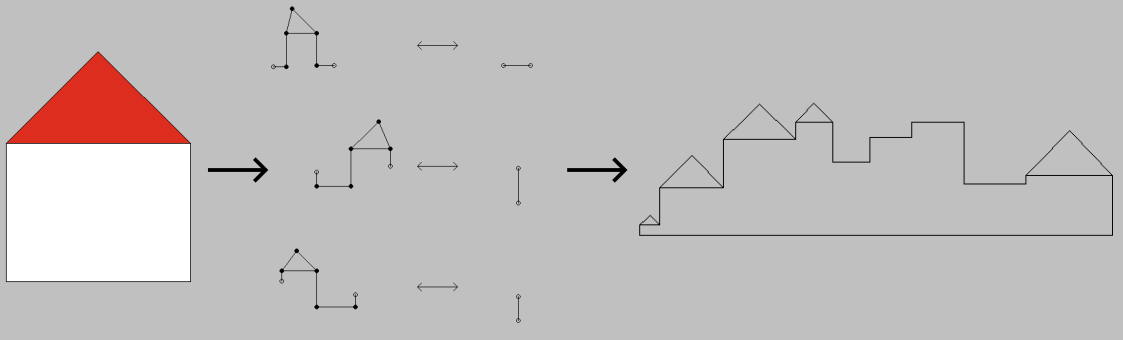
\includegraphics[width=\textwidth]{images/house_success.png}
    \caption{Erfolgreicher Durchlauf mit Input-Datei \code{house.mesh}.}
    \label{fig:house_success}
\end{figure}

Für den in Abbildung \ref{fig:square_double_success} dargestellten Durchlauf verwendete Parameter: \code{seed = 77}, \code{maxGeneration = 3}, \code{iterations = 7},
\code{maxTries = 100}, \code{minRandVal = 10}, \code{maxRandVal = 100}. Die Ergebnisse entsprechen den Erwartungen.
\begin{figure}[H]
    \centering
    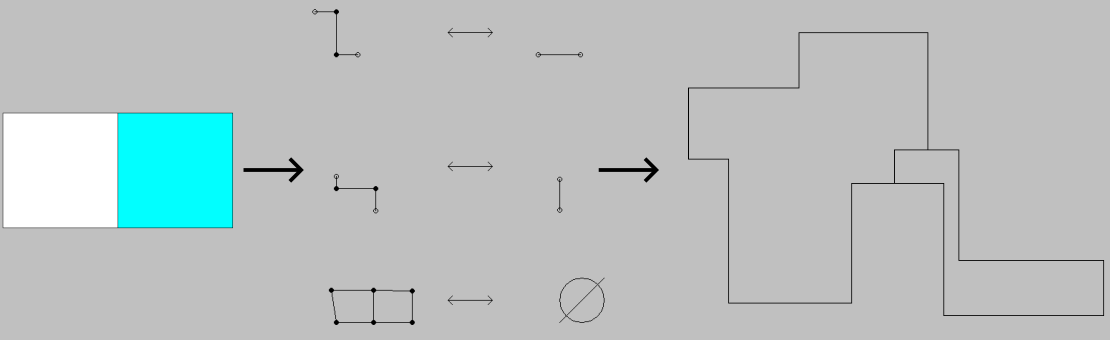
\includegraphics[width=\textwidth]{images/square_double_success.png}
    \caption{Erfolgreicher Durchlauf mit Input-Datei \code{square\_double.mesh}.}
    \label{fig:square_double_success}
\end{figure}

Für den in Abbildung \ref{fig:square_success} dargestellten Durchlauf verwendete Parameter: \code{seed = 5555}, \code{maxGeneration = 3}, \code{iterations = 5},
\code{maxTries = 100}, \code{minRandVal = 10}, \code{maxRandVal = 10}. Die Ergebnisse entsprechen den Erwartungen. Durch das Limitieren der Zufallszahlen auf nur
exakt einen Wert enthält der Output sehr viele Kanten mit der gleichen Kantenlänge und nimmt somit eine regelmäßige Form an. Es wirkt, als wäre der Output auf
Basis eines Gitters modelliert worden.
\begin{figure}[H]
    \centering
    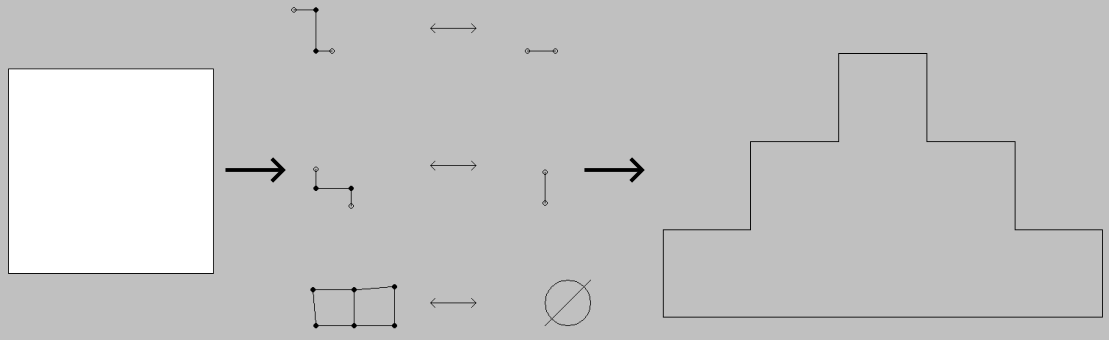
\includegraphics[width=\textwidth]{images/square_success.png}
    \caption{Erfolgreicher Durchlauf mit Input-Datei \code{square.mesh}.}
    \label{fig:square_success}
\end{figure}

Für den in Abbildung \ref{fig:rhombus_success} dargestellten Durchlauf verwendete Parameter: \code{seed = 123}, \code{maxGeneration = 3}, \code{iterations = 10},
\code{maxTries = 100}, \code{minRandVal = 10}, \code{maxRandVal = 70}. Die Ergebnisse entsprechen den Erwartungen.
\begin{figure}[H]
    \centering
    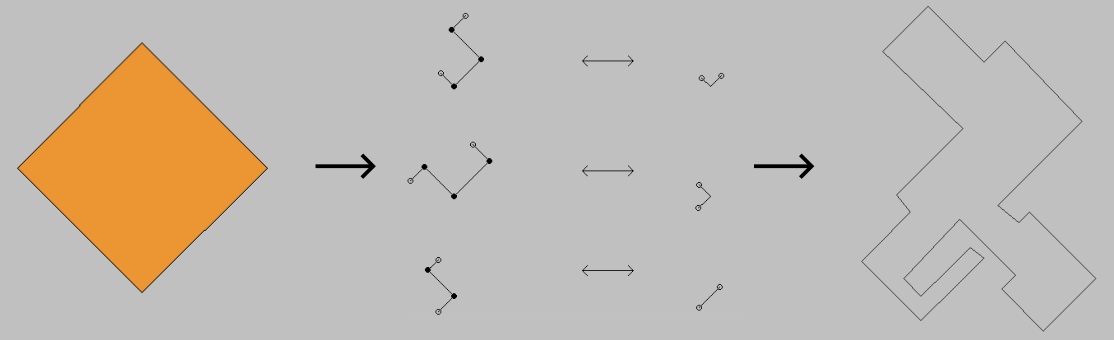
\includegraphics[width=\textwidth]{images/rhombus_success.png}
    \caption{Erfolgreicher Durchlauf mit Input-Datei \code{rhombus.mesh}.}
    \label{fig:rhombus_success}
\end{figure}

\subsection{Fehlerhafte Durchläufe}

Für den in Abbildung \ref{fig:house_fail} dargestellten Durchlauf verwendete Parameter: \code{seed = 337}, \code{maxGeneration = 7}, \code{iterations = 7},
\code{maxTries = 100}, \code{minRandVal = 10}, \code{maxRandVal = 100}. Die Ergebnisse entsprechen nicht den Erwartungen. Alle dargestellten Kantenwinkel
lassen sich zwar im Input wiederfinden und es wirkt so, als wäre die erzeugte Outputstruktur zumindest lokal ähnlich zum Input. Das Ergebnis ist jedoch
trotzdem fehlerhaft, da sich einige der Kanten überschneiden.
\begin{figure}[H]
    \centering
    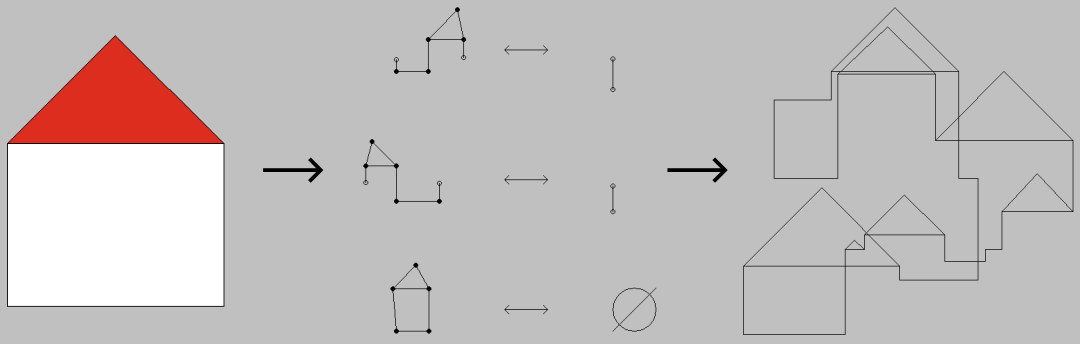
\includegraphics[width=\textwidth]{images/house_fail.png}
    \caption{Fehlerhafter Durchlauf mit Input-Datei \code{house.mesh}.}
    \label{fig:house_fail}
\end{figure}

Für den in Abbildung \ref{fig:octagon_fail} dargestellten Durchlauf verwendete Parameter: \code{seed = 445}, \code{maxGeneration = 2}, \code{iterations = 7},
\code{maxTries = 10}, \code{minRandVal = 10}, \code{maxRandVal = 100}. Diesmal ist der dargestellte Output planar, jedoch liegt hier keine lokale Ähnlichkeit
vor. Die Kantenwinkel stimmen zwar alle mit den Kantenwinkeln im Input überein, jedoch unterscheidet sich die Topologie der beiden Strukturen an einigen Stellen.
Einige der Knoten in der Outputstruktur (an den ``Spitzen'') lassen sich nicht im Input wiederfinden.
\begin{figure}[H]
    \centering
    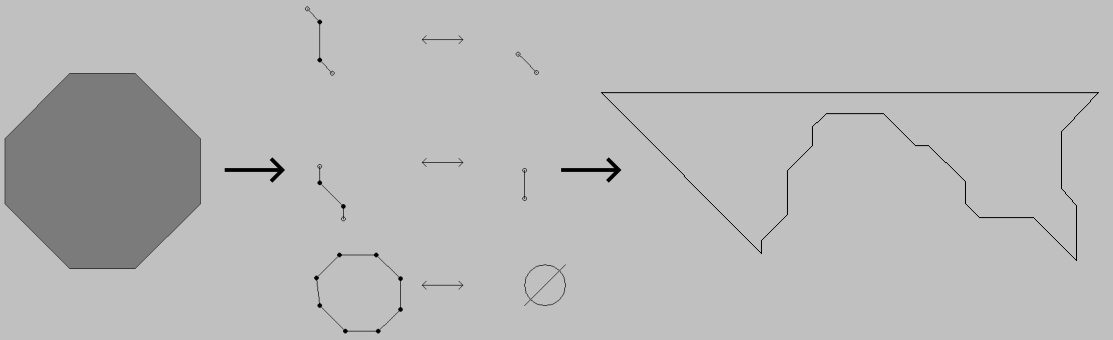
\includegraphics[width=\textwidth]{images/octagon_fail.png}
    \caption{Fehlerhafter Durchlauf mit Input-Datei \code{octagon.mesh}.}
    \label{fig:octagon_fail}
\end{figure}

Für den in Abbildung \ref{fig:triangle_fail} dargestellten Durchlauf verwendete Parameter: \code{seed = 23456}, \code{maxGeneration = 30}, \code{iterations = 3},
\code{maxTries = 100}, \code{minRandVal = 10}, \code{maxRandVal = 100}. Der Output entspricht den geforderten Eigenschaften, ist sowohl zum Input lokal
ähnlich als auch planar und somit nicht fehlerhaft. Trotzdem ist das Ergebnis unbrauchbar, da sich der Output kaum vom Input unterscheidet. Der Output
besitzt zwar andere Kantenlängen, ist strukturell allerdings exakt gleich aufgebaut. Trotz der hohen Anzahl an zugelassenen Generationen konnte das Verfahren
lediglich nur eine einzige Starter-Regel für die Grammatik ableiten (beide dargestellten Starter-Regeln sind identisch). Aus dieser Grammatik kann keine
hohe Vielfalt an Ergebnissen erzeugt werden.
\begin{figure}[H]  
    \centering  
    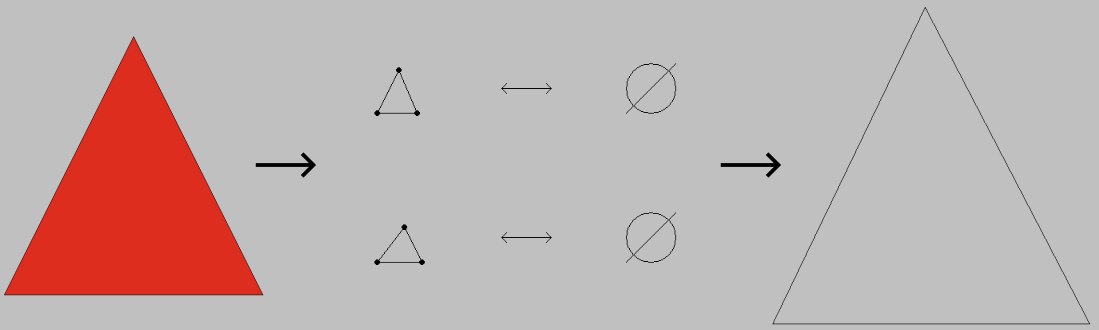
\includegraphics[width=\textwidth]{images/triangle_fail.png}
    \caption{Ungenügender Durchlauf mit Input-Datei \code{triangle.mesh}.}
    \label{fig:triangle_fail}
\end{figure}

\section{Auswertung der Ergebnisse}
Allgemein sind die Ergebnisse durchaus zufriedenstellend. Die erzeugten Strukturen erfüllen zwar in vielen Fällen nicht die Anforderungen an die lokale
Ähnlichkeit und können auch oft nicht ohne Überschneidungen einiger der Kanten dargestellt werden, jedoch wird durch die von uns implementierte Software
klar demonstriert, dass dieses Verfahren grundsätzlich funktioniert. Auch wenn es dabei noch viele Probleme gibt, die behoben werden müssen um dieses
Verfahren wirklich in der Praxis einsetzen zu können, erfüllt die entwickelte Anwendung voll und ganz ihren Zweck als Prototyp.

% @author Benjamin Schröder
%
\chapter{Fazit} % Auswerten der gesamten Arbeit
Abschließend soll diese Arbeit kurz reflektiert werden. Dazu fassen wir die gewonnenen Erkenntnisse zusammen und geben
anschließend einen Ausblick auf mögliche Verbesserungen und Erweiterungsmöglichkeiten des vorgestellten Ansatzes und
seiner Umsetzung.

\section{Zusammenfassung}

\section{Verbesserungsansätze und Erweiterungsmöglichkeiten}


%\bibliographystyle{plain}
\bibliographystyle{dinat}
\bibliography{literature}

% Appendix
\appendix
% !TEX root = ../thesis.tex
% appendix example chapter
% @author Thomas Lehmann
%

\chapter{Anhang}

\section{Verwendete Hilfsmittel}
In der Tabelle \ref{tab:tooling} sind die im Rahmen der Bearbeitung des Themas der \IthesisKindDE~verwendeten Werkzeuge und Hilfsmittel aufgelistet.

\begin{table}[h!]
\caption{Verwendete Hilfsmittel und Werkzeuge}
\begin{tabular}{|l|l|}
\hline 
\rowcolor{lightgray} Tool & Verwendung \\
\hline
\LaTeX & Textsatz- und Layout-Werkzeug verwendet zur Erstellung dieses Dokuments \\
\hline
 & \\
\hline
\end{tabular}
\label{tab:tooling}
\end{table}



\IGlossary

\Istatement

\end{document}

% compile using the following commands:
%
% pdflatex thesis.tex
% bibtex thesis
% makeglossaries thesis
% pdflatex thesis.tex
% pdflatex thesis.tex
